% Options for packages loaded elsewhere
\PassOptionsToPackage{unicode}{hyperref}
\PassOptionsToPackage{hyphens}{url}
%
\documentclass[
]{article}
\usepackage{amsmath,amssymb}
\usepackage{lmodern}
\usepackage{ifxetex,ifluatex}
\ifnum 0\ifxetex 1\fi\ifluatex 1\fi=0 % if pdftex
  \usepackage[T1]{fontenc}
  \usepackage[utf8]{inputenc}
  \usepackage{textcomp} % provide euro and other symbols
\else % if luatex or xetex
  \usepackage{unicode-math}
  \defaultfontfeatures{Scale=MatchLowercase}
  \defaultfontfeatures[\rmfamily]{Ligatures=TeX,Scale=1}
\fi
% Use upquote if available, for straight quotes in verbatim environments
\IfFileExists{upquote.sty}{\usepackage{upquote}}{}
\IfFileExists{microtype.sty}{% use microtype if available
  \usepackage[]{microtype}
  \UseMicrotypeSet[protrusion]{basicmath} % disable protrusion for tt fonts
}{}
\makeatletter
\@ifundefined{KOMAClassName}{% if non-KOMA class
  \IfFileExists{parskip.sty}{%
    \usepackage{parskip}
  }{% else
    \setlength{\parindent}{0pt}
    \setlength{\parskip}{6pt plus 2pt minus 1pt}}
}{% if KOMA class
  \KOMAoptions{parskip=half}}
\makeatother
\usepackage{xcolor}
\IfFileExists{xurl.sty}{\usepackage{xurl}}{} % add URL line breaks if available
\IfFileExists{bookmark.sty}{\usepackage{bookmark}}{\usepackage{hyperref}}
\hypersetup{
  pdftitle={西南大学 2022: STATS 201 Assignment 3},
  pdfauthor={Runze liao 222020321102007},
  hidelinks,
  pdfcreator={LaTeX via pandoc}}
\urlstyle{same} % disable monospaced font for URLs
\usepackage[margin=1in]{geometry}
\usepackage{color}
\usepackage{fancyvrb}
\newcommand{\VerbBar}{|}
\newcommand{\VERB}{\Verb[commandchars=\\\{\}]}
\DefineVerbatimEnvironment{Highlighting}{Verbatim}{commandchars=\\\{\}}
% Add ',fontsize=\small' for more characters per line
\usepackage{framed}
\definecolor{shadecolor}{RGB}{248,248,248}
\newenvironment{Shaded}{\begin{snugshade}}{\end{snugshade}}
\newcommand{\AlertTok}[1]{\textcolor[rgb]{0.94,0.16,0.16}{#1}}
\newcommand{\AnnotationTok}[1]{\textcolor[rgb]{0.56,0.35,0.01}{\textbf{\textit{#1}}}}
\newcommand{\AttributeTok}[1]{\textcolor[rgb]{0.77,0.63,0.00}{#1}}
\newcommand{\BaseNTok}[1]{\textcolor[rgb]{0.00,0.00,0.81}{#1}}
\newcommand{\BuiltInTok}[1]{#1}
\newcommand{\CharTok}[1]{\textcolor[rgb]{0.31,0.60,0.02}{#1}}
\newcommand{\CommentTok}[1]{\textcolor[rgb]{0.56,0.35,0.01}{\textit{#1}}}
\newcommand{\CommentVarTok}[1]{\textcolor[rgb]{0.56,0.35,0.01}{\textbf{\textit{#1}}}}
\newcommand{\ConstantTok}[1]{\textcolor[rgb]{0.00,0.00,0.00}{#1}}
\newcommand{\ControlFlowTok}[1]{\textcolor[rgb]{0.13,0.29,0.53}{\textbf{#1}}}
\newcommand{\DataTypeTok}[1]{\textcolor[rgb]{0.13,0.29,0.53}{#1}}
\newcommand{\DecValTok}[1]{\textcolor[rgb]{0.00,0.00,0.81}{#1}}
\newcommand{\DocumentationTok}[1]{\textcolor[rgb]{0.56,0.35,0.01}{\textbf{\textit{#1}}}}
\newcommand{\ErrorTok}[1]{\textcolor[rgb]{0.64,0.00,0.00}{\textbf{#1}}}
\newcommand{\ExtensionTok}[1]{#1}
\newcommand{\FloatTok}[1]{\textcolor[rgb]{0.00,0.00,0.81}{#1}}
\newcommand{\FunctionTok}[1]{\textcolor[rgb]{0.00,0.00,0.00}{#1}}
\newcommand{\ImportTok}[1]{#1}
\newcommand{\InformationTok}[1]{\textcolor[rgb]{0.56,0.35,0.01}{\textbf{\textit{#1}}}}
\newcommand{\KeywordTok}[1]{\textcolor[rgb]{0.13,0.29,0.53}{\textbf{#1}}}
\newcommand{\NormalTok}[1]{#1}
\newcommand{\OperatorTok}[1]{\textcolor[rgb]{0.81,0.36,0.00}{\textbf{#1}}}
\newcommand{\OtherTok}[1]{\textcolor[rgb]{0.56,0.35,0.01}{#1}}
\newcommand{\PreprocessorTok}[1]{\textcolor[rgb]{0.56,0.35,0.01}{\textit{#1}}}
\newcommand{\RegionMarkerTok}[1]{#1}
\newcommand{\SpecialCharTok}[1]{\textcolor[rgb]{0.00,0.00,0.00}{#1}}
\newcommand{\SpecialStringTok}[1]{\textcolor[rgb]{0.31,0.60,0.02}{#1}}
\newcommand{\StringTok}[1]{\textcolor[rgb]{0.31,0.60,0.02}{#1}}
\newcommand{\VariableTok}[1]{\textcolor[rgb]{0.00,0.00,0.00}{#1}}
\newcommand{\VerbatimStringTok}[1]{\textcolor[rgb]{0.31,0.60,0.02}{#1}}
\newcommand{\WarningTok}[1]{\textcolor[rgb]{0.56,0.35,0.01}{\textbf{\textit{#1}}}}
\usepackage{graphicx}
\makeatletter
\def\maxwidth{\ifdim\Gin@nat@width>\linewidth\linewidth\else\Gin@nat@width\fi}
\def\maxheight{\ifdim\Gin@nat@height>\textheight\textheight\else\Gin@nat@height\fi}
\makeatother
% Scale images if necessary, so that they will not overflow the page
% margins by default, and it is still possible to overwrite the defaults
% using explicit options in \includegraphics[width, height, ...]{}
\setkeys{Gin}{width=\maxwidth,height=\maxheight,keepaspectratio}
% Set default figure placement to htbp
\makeatletter
\def\fps@figure{htbp}
\makeatother
\setlength{\emergencystretch}{3em} % prevent overfull lines
\providecommand{\tightlist}{%
  \setlength{\itemsep}{0pt}\setlength{\parskip}{0pt}}
\setcounter{secnumdepth}{-\maxdimen} % remove section numbering
\ifluatex
  \usepackage{selnolig}  % disable illegal ligatures
\fi

\title{西南大学 2022: STATS 201 Assignment 3}
\author{Runze liao 222020321102007}
\date{2022/5/31}

\begin{document}
\maketitle

\hypertarget{question-1}{%
\section{Question 1}\label{question-1}}

\hypertarget{question-of-interestgoal-of-the-study}{%
\subsection{Question of interest/goal of the
study}\label{question-of-interestgoal-of-the-study}}

A leading car distributor invited visitors to its website to complete a
survey to learn about how much they were willing to spend on a new car.
It was of interest to see how this depended on the participant's annual
income, marital status, dependents, gender and age. The variables in
\texttt{CarSpend.txt} are:

\begin{itemize}
\tightlist
\item
  \texttt{MaxSpend}: Maximum participant will spend on a new car (\$)
\item
  \texttt{Income}: Annual income (\$)
\item
  \texttt{Partner}: 1=in a partnership, 0=single
\item
  \texttt{Dependents}: 1=have financial dependents, 0=no financial
  dependents
\item
  \texttt{Sex}: M or F
\item
  \texttt{Age}: Age (years)
\end{itemize}

\hypertarget{read-in-and-inspect-the-data-using-a-pairs20x-plot}{%
\subsection{Read in and inspect the data using a pairs20x
plot}\label{read-in-and-inspect-the-data-using-a-pairs20x-plot}}

\begin{Shaded}
\begin{Highlighting}[]
\FunctionTok{pairs20x}\NormalTok{(CarSpend.df[,}\FunctionTok{c}\NormalTok{(}\DecValTok{1}\NormalTok{,}\DecValTok{2}\NormalTok{,}\DecValTok{3}\NormalTok{,}\DecValTok{4}\NormalTok{,}\DecValTok{5}\NormalTok{,}\DecValTok{6}\NormalTok{)])}
\end{Highlighting}
\end{Shaded}

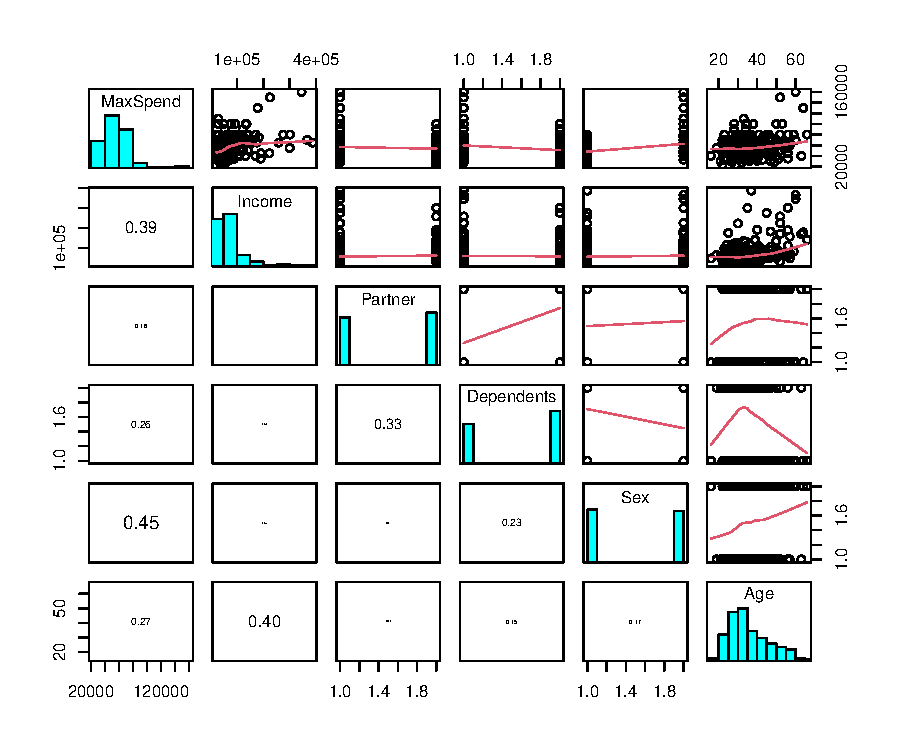
\includegraphics{STATS201_2022_SWU_A3_files/figure-latex/unnamed-chunk-2-1.pdf}

\hypertarget{comment-on-the-pairs20x-plot}{%
\subsection{Comment on the pairs20x
plot}\label{comment-on-the-pairs20x-plot}}

From the pairs20x plot we can see that the relation between the Partner,
Dependents and Sex is quiet linear, since it is the factor variable.
However, with the Income and Age, they are not having strong
relationship between them. And the explanatory variables seems have
little interaction between each other.

\hypertarget{why-log-the-responses}{%
\subsection{Why log the responses?}\label{why-log-the-responses}}

\textbf{\texttt{In\ the\ analysis\ below\ you\ will\ log\ the\ response\ variable.\ Provide\ at\ least\ one\ reason\ why\ this\ is\ a\ sensible\ thing\ to\ do}}
With the pairs20x plot, we can indicate that it is used multiplicative
linear model to fit a nice model. As needs to fit the linear model, we
need log transformation to turn the multiplicative effects in to
additive effect. So we choose to log the responses variable.

\hypertarget{fit-model-and-check-assumptions}{%
\subsection{Fit model and check
assumptions}\label{fit-model-and-check-assumptions}}

\begin{Shaded}
\begin{Highlighting}[]
\NormalTok{CarSpend.fit }\OtherTok{=} \FunctionTok{lm}\NormalTok{(MaxSpend}\SpecialCharTok{\textasciitilde{}}\NormalTok{Income}\SpecialCharTok{+}\NormalTok{Partner}\SpecialCharTok{+}\NormalTok{Dependents}\SpecialCharTok{+}\NormalTok{Sex}\SpecialCharTok{+}\NormalTok{Age, }\AttributeTok{data =}\NormalTok{ CarSpend.df)}
\end{Highlighting}
\end{Shaded}

we can see that the residual plot is quiet strange.

\begin{Shaded}
\begin{Highlighting}[]
\NormalTok{CarSpend.fit2 }\OtherTok{=} \FunctionTok{lm}\NormalTok{(}\FunctionTok{log}\NormalTok{(MaxSpend)}\SpecialCharTok{\textasciitilde{}}\NormalTok{Income}\SpecialCharTok{+}\NormalTok{Partner}\SpecialCharTok{+}\NormalTok{Dependents}\SpecialCharTok{+}\NormalTok{Sex}\SpecialCharTok{+}\NormalTok{Age, }\AttributeTok{data =}\NormalTok{ CarSpend.df)}
\FunctionTok{plot}\NormalTok{(CarSpend.fit2 , }\AttributeTok{which =} \DecValTok{1}\NormalTok{)}
\end{Highlighting}
\end{Shaded}

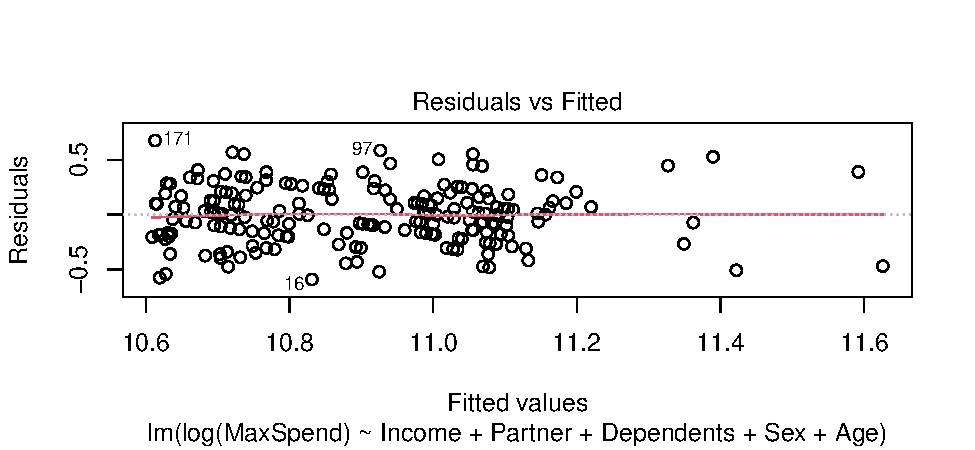
\includegraphics{STATS201_2022_SWU_A3_files/figure-latex/unnamed-chunk-4-1.pdf}

\begin{Shaded}
\begin{Highlighting}[]
\FunctionTok{normcheck}\NormalTok{(CarSpend.fit2)}
\end{Highlighting}
\end{Shaded}

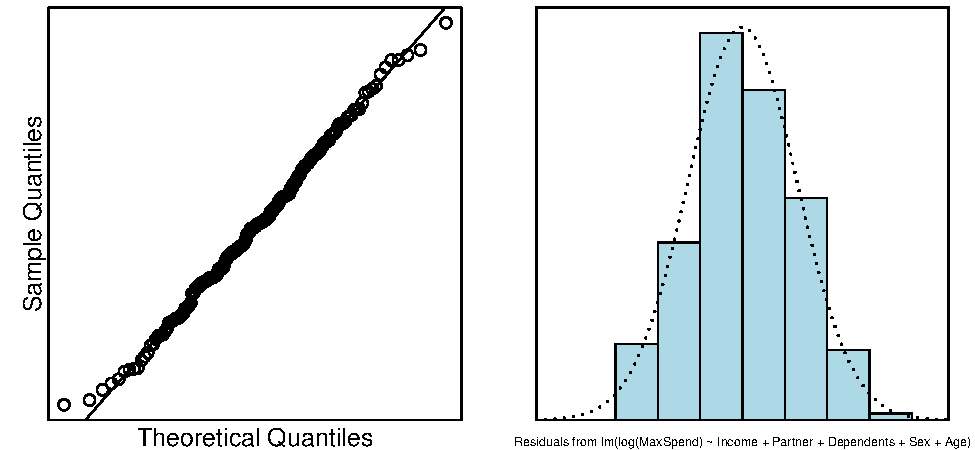
\includegraphics{STATS201_2022_SWU_A3_files/figure-latex/unnamed-chunk-4-2.pdf}

\begin{Shaded}
\begin{Highlighting}[]
\FunctionTok{cooks20x}\NormalTok{(CarSpend.fit2)}
\end{Highlighting}
\end{Shaded}

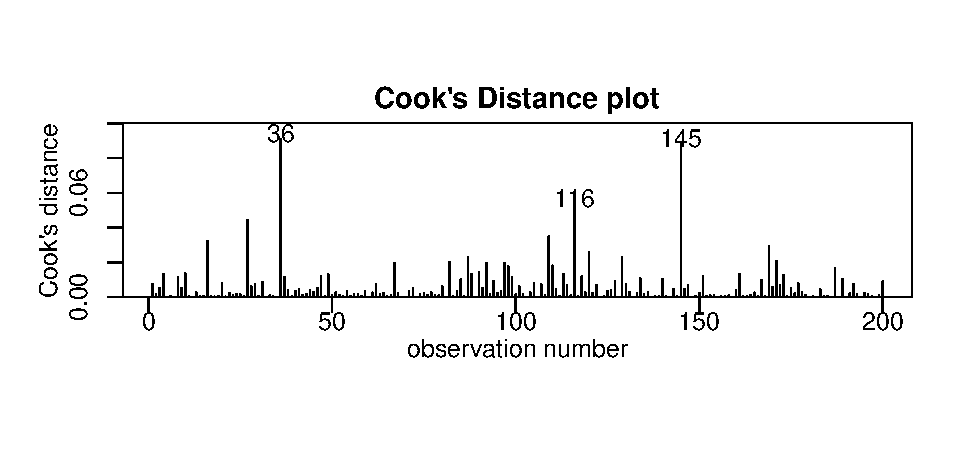
\includegraphics{STATS201_2022_SWU_A3_files/figure-latex/unnamed-chunk-4-3.pdf}

From the residual plot, we can see that we've been satisfied the eov
assumption, the normcheck is fine, No too strong influence point,
however, point 36, 145 seems strange, but we will keep it. All
assumption were satisfied, let us see the summary part.

\begin{Shaded}
\begin{Highlighting}[]
\FunctionTok{summary}\NormalTok{(CarSpend.fit2)}
\end{Highlighting}
\end{Shaded}

\begin{verbatim}
## 
## Call:
## lm(formula = log(MaxSpend) ~ Income + Partner + Dependents + 
##     Sex + Age, data = CarSpend.df)
## 
## Residuals:
##      Min       1Q   Median       3Q      Max 
## -0.59125 -0.17113 -0.00126  0.17831  0.67695 
## 
## Coefficients:
##               Estimate Std. Error t value Pr(>|t|)    
## (Intercept)  1.069e+01  7.581e-02 140.950  < 2e-16 ***
## Income       1.620e-06  3.357e-07   4.826 2.81e-06 ***
## Partner1    -8.225e-02  3.994e-02  -2.059   0.0408 *  
## Dependents1 -7.246e-02  4.140e-02  -1.750   0.0817 .  
## SexM         2.883e-01  3.865e-02   7.460 2.83e-12 ***
## Age          9.817e-04  2.010e-03   0.488   0.6258    
## ---
## Signif. codes:  0 '***' 0.001 '**' 0.01 '*' 0.05 '.' 0.1 ' ' 1
## 
## Residual standard error: 0.261 on 194 degrees of freedom
## Multiple R-squared:  0.3748, Adjusted R-squared:  0.3587 
## F-statistic: 23.26 on 5 and 194 DF,  p-value: < 2.2e-16
\end{verbatim}

By applying the Occam's Razor, we choose to remove the coefficients that
are out of significant at the 5\% level(those p-value \textgreater{}
0.05), which means we will remove the Dependents, Age. keeping the
Income and Partner, Sex to fit a latest model.

\begin{Shaded}
\begin{Highlighting}[]
\NormalTok{CarSpend.fit3 }\OtherTok{=} \FunctionTok{lm}\NormalTok{(}\FunctionTok{log}\NormalTok{(MaxSpend)}\SpecialCharTok{\textasciitilde{}}\NormalTok{Income}\SpecialCharTok{+}\NormalTok{Partner}\SpecialCharTok{+}\NormalTok{Sex, }\AttributeTok{data =}\NormalTok{ CarSpend.df)}
\FunctionTok{summary}\NormalTok{(CarSpend.fit3)}
\end{Highlighting}
\end{Shaded}

\begin{verbatim}
## 
## Call:
## lm(formula = log(MaxSpend) ~ Income + Partner + Sex, data = CarSpend.df)
## 
## Residuals:
##      Min       1Q   Median       3Q      Max 
## -0.59644 -0.17584 -0.00019  0.16949  0.66728 
## 
## Coefficients:
##               Estimate Std. Error t value Pr(>|t|)    
## (Intercept)  1.067e+01  3.970e-02 268.850  < 2e-16 ***
## Income       1.719e-06  3.086e-07   5.571 8.28e-08 ***
## Partner1    -1.049e-01  3.720e-02  -2.820  0.00529 ** 
## SexM         3.090e-01  3.719e-02   8.308 1.59e-14 ***
## ---
## Signif. codes:  0 '***' 0.001 '**' 0.01 '*' 0.05 '.' 0.1 ' ' 1
## 
## Residual standard error: 0.2621 on 196 degrees of freedom
## Multiple R-squared:  0.3632, Adjusted R-squared:  0.3534 
## F-statistic: 37.26 on 3 and 196 DF,  p-value: < 2.2e-16
\end{verbatim}

All the assumptions seem to be satisfied, we have evidence to keep all
the coefficients(p-value \textless{} 0.05), it is a good fit model, we
can trust our final model.
\textbf{\texttt{Fit\ a\ linear\ regression\ model\ for\ log(MaxSpend)\ that\ contains\ the\ five\ explanatory\ terms\ log(Income),\ Partner,\ Dependents,\ Sex,\ Age.\ Then,\ apply\ Occam\textquotesingle{}s\ Razor\ −\ that\ is,\ simplify\ the\ model\ by\ successively\ removing\ the\ least\ significant\ term\ until\ all\ are\ significant\ at\ the\ 5\%\ level.}}

\begin{Shaded}
\begin{Highlighting}[]
\FunctionTok{exp}\NormalTok{(}\FunctionTok{confint}\NormalTok{(CarSpend.fit3))}
\end{Highlighting}
\end{Shaded}

\begin{verbatim}
##                    2.5 %       97.5 %
## (Intercept) 3.996638e+04 4.674175e+04
## Income      1.000001e+00 1.000002e+00
## Partner1    8.367306e-01 9.689525e-01
## SexM        1.265721e+00 1.465719e+00
\end{verbatim}

\hypertarget{method-and-assumption-checks}{%
\subsection{Method and Assumption
Checks}\label{method-and-assumption-checks}}

By having looked at the Pair20 plot, we got that the Max Spend in car
were related to serveral explanatory variables, So we construct a
multiple linear regression model with a suitable selection of the
explanatory variables, moreover, we choose to log the responses variable
by having the transformation turn the multiplicative effects in to
additive effect.

Furthermore, we decide to keep the Income and Partner, Sex to fit a
latest model, deleting the the Dependents, Age, because they were out of
the 95\% confidence interval.

So our final model is:
\[MaxSpend_i = \beta_0 + \beta_1 \times Income_i + \beta_2 \times Partner_i + \beta_3 \times Sex_i + \epsilon_i \]

where \(\epsilon_i\) \textasciitilde{} \(iid.N(0,\sigma^2)\). Here our
indicator variable takes value 1 if the Sex is Male.

Our model explains about 36.3\% of the variability in people's max spend
in cars.

\hypertarget{executive-summary}{%
\subsection{Executive Summary}\label{executive-summary}}

We wanted to have a model to explain how much visitors want to spend on
a new car depending on the income, marital status, dependents, gender
and age.\\
We have estimated that: - The Male would choose to spend 1.26 to 1.46
than the Female on a new car.

\begin{itemize}
\item
  People who got married are more likely to spend 0.84 to 0.97 than
  those who not.
\item
  For each one more in thier Income, we estmated that they would like
  spending incresing 1 than before.
\end{itemize}

\newpage

\hypertarget{question-2}{%
\section{Question 2}\label{question-2}}

\hypertarget{question-of-interestgoal-of-the-study-1}{%
\subsection{Question of interest/goal of the
study}\label{question-of-interestgoal-of-the-study-1}}

A company was interested in assessing 3 different display panels used by
air traffic controllers. An experiment was conducted by simulating 4
different emergency conditions with 4 qualified air traffic controllers
randomly assigned to each display/emergency combination. The time (in
seconds) required to stabilise the emergency condition was recorded. The
data are stored in the text file \texttt{airtraffic.txt}, which contains
the variables:

\begin{itemize}
\tightlist
\item
  \texttt{time}: the time required to stabilise the emergency condition
  (seconds)
\item
  \texttt{display}: the display panel: 1, 2 or 3
\item
  \texttt{emergency}: the simulated emergency condition: A, B, C or D
\end{itemize}

We are \textbf{only interested in which display has the lowest time} to
stabilise the emergencies, by how much lower it is than the other
displays and whether answer this depends on the type of emergency
simulated. You should \emph{NOT} quantify extraneous information.

\hypertarget{read-in-and-plot-the-data}{%
\subsection{Read in and plot the data}\label{read-in-and-plot-the-data}}

\begin{Shaded}
\begin{Highlighting}[]
\NormalTok{airtraffic.df }\OtherTok{=} \FunctionTok{read.table}\NormalTok{(}\AttributeTok{file =} \StringTok{"airtraffic.txt"}\NormalTok{, }\AttributeTok{header =} \ConstantTok{TRUE}\NormalTok{)}
\NormalTok{airtraffic.df}\SpecialCharTok{$}\NormalTok{display }\OtherTok{=} \FunctionTok{as.factor}\NormalTok{(airtraffic.df}\SpecialCharTok{$}\NormalTok{display)}
\NormalTok{airtraffic.df}\SpecialCharTok{$}\NormalTok{emergency }\OtherTok{=} \FunctionTok{as.factor}\NormalTok{(airtraffic.df}\SpecialCharTok{$}\NormalTok{emergency)}
\FunctionTok{interactionPlots}\NormalTok{(time}\SpecialCharTok{\textasciitilde{}}\NormalTok{display}\SpecialCharTok{+}\NormalTok{emergency, }\AttributeTok{data =}\NormalTok{ airtraffic.df)}
\end{Highlighting}
\end{Shaded}

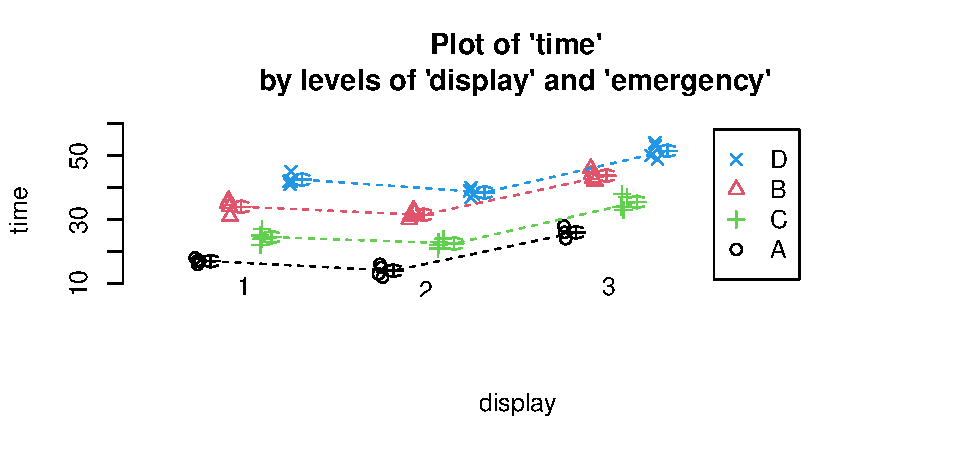
\includegraphics{STATS201_2022_SWU_A3_files/figure-latex/unnamed-chunk-8-1.pdf}

\hypertarget{comment-on-the-plot}{%
\subsection{Comment on the plot}\label{comment-on-the-plot}}

By looking at the interaction plot of display and emergency, we see
those parallel lines, which indicating that the two explanatory
variables have no interaction. And on average we can see that with the
same emergency, time of display 3 \textgreater{} 1 \textgreater{} 2, and
with the same display, time of emergency D \textgreater{} B
\textgreater{} C \textgreater{} A.

\hypertarget{fit-model-check-assumptions-and-do-inference-cis-etc}{%
\subsection{Fit model, check assumptions and do inference (CIs
etc)}\label{fit-model-check-assumptions-and-do-inference-cis-etc}}

So we choose to fit a model with no interaction and a two-ANOVA model.

\begin{Shaded}
\begin{Highlighting}[]
\NormalTok{airtraffic.fit }\OtherTok{=} \FunctionTok{lm}\NormalTok{(time}\SpecialCharTok{\textasciitilde{}}\NormalTok{display}\SpecialCharTok{+}\NormalTok{emergency, }\AttributeTok{data =}\NormalTok{ airtraffic.df)}
\end{Highlighting}
\end{Shaded}

\begin{Shaded}
\begin{Highlighting}[]
\FunctionTok{plot}\NormalTok{(airtraffic.fit,}\AttributeTok{which =} \DecValTok{1}\NormalTok{)}
\end{Highlighting}
\end{Shaded}

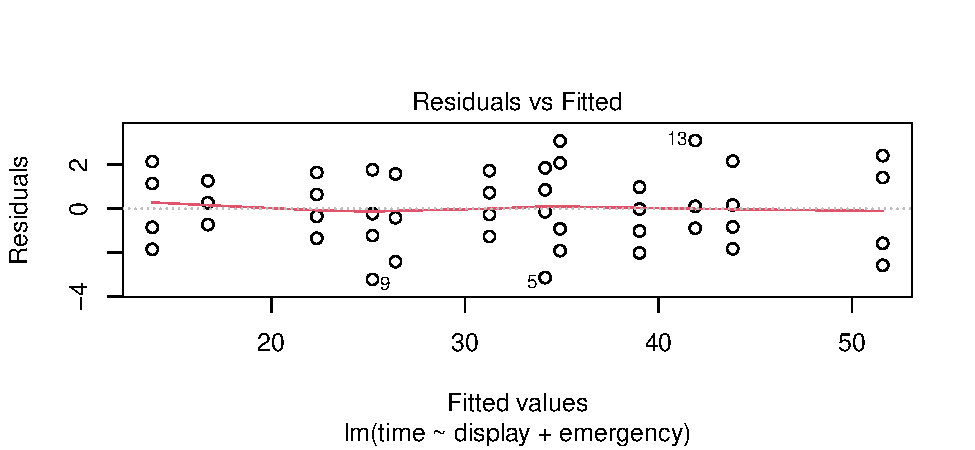
\includegraphics{STATS201_2022_SWU_A3_files/figure-latex/unnamed-chunk-10-1.pdf}

\begin{Shaded}
\begin{Highlighting}[]
\FunctionTok{normcheck}\NormalTok{(airtraffic.fit)}
\end{Highlighting}
\end{Shaded}

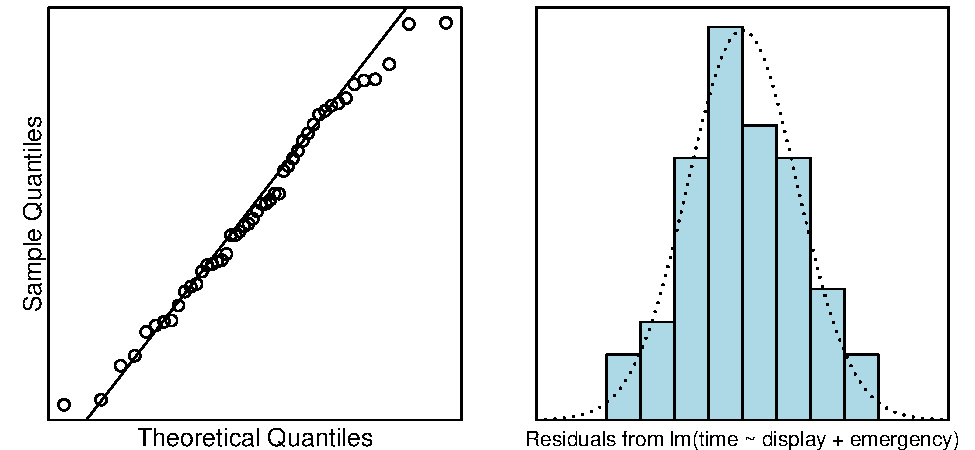
\includegraphics{STATS201_2022_SWU_A3_files/figure-latex/unnamed-chunk-10-2.pdf}

\begin{Shaded}
\begin{Highlighting}[]
\FunctionTok{cooks20x}\NormalTok{(airtraffic.fit)}
\end{Highlighting}
\end{Shaded}

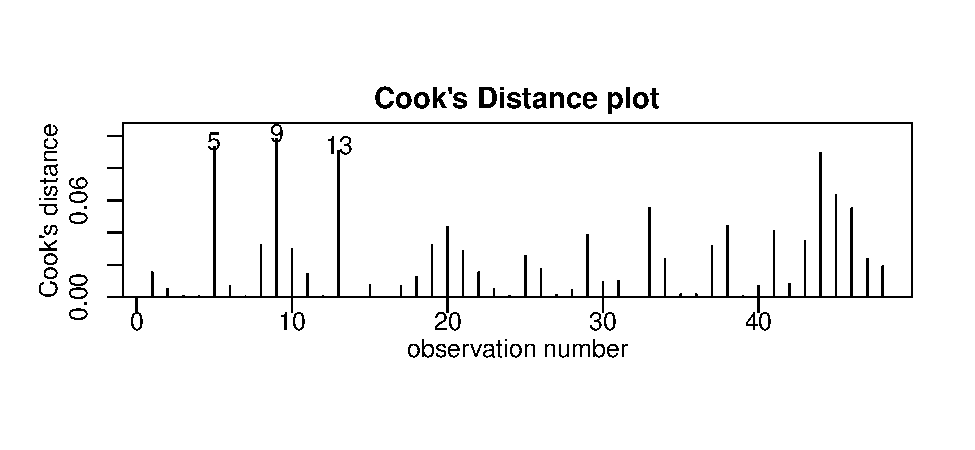
\includegraphics{STATS201_2022_SWU_A3_files/figure-latex/unnamed-chunk-10-3.pdf}
A little bit strange in the residual plot, and the normal check is
strange too, however, we will tolerant it. From the cooks plot, no
strong influence point, it seems it is a good model, and satisfy most of
the assumptions. We can trust our model.

\begin{Shaded}
\begin{Highlighting}[]
\FunctionTok{summary}\NormalTok{(airtraffic.fit)}
\end{Highlighting}
\end{Shaded}

\begin{verbatim}
## 
## Call:
## lm(formula = time ~ display + emergency, data = airtraffic.df)
## 
## Residuals:
##     Min      1Q  Median      3Q     Max 
## -3.2292 -1.0729 -0.0833  1.3073  3.1042 
## 
## Coefficients:
##             Estimate Std. Error t value Pr(>|t|)    
## (Intercept)  16.7292     0.6008  27.844  < 2e-16 ***
## display2     -2.8750     0.6008  -4.785 2.13e-05 ***
## display3      9.6875     0.6008  16.124  < 2e-16 ***
## emergencyB   17.4167     0.6938  25.104  < 2e-16 ***
## emergencyC    8.5000     0.6938  12.252 1.87e-15 ***
## emergencyD   25.1667     0.6938  36.275  < 2e-16 ***
## ---
## Signif. codes:  0 '***' 0.001 '**' 0.01 '*' 0.05 '.' 0.1 ' ' 1
## 
## Residual standard error: 1.699 on 42 degrees of freedom
## Multiple R-squared:  0.979,  Adjusted R-squared:  0.9765 
## F-statistic: 392.3 on 5 and 42 DF,  p-value: < 2.2e-16
\end{verbatim}

All Coefficients are in 95\% confidence interval(p-value \textless{}
0.05), it seems that it is a nice model we can trust.

\begin{Shaded}
\begin{Highlighting}[]
\FunctionTok{confint}\NormalTok{(airtraffic.fit)}
\end{Highlighting}
\end{Shaded}

\begin{verbatim}
##                 2.5 %    97.5 %
## (Intercept) 15.516659 17.941675
## display2    -4.087508 -1.662492
## display3     8.474992 10.900008
## emergencyB  16.016583 18.816750
## emergencyC   7.099916  9.900084
## emergencyD  23.766583 26.566750
\end{verbatim}

\begin{Shaded}
\begin{Highlighting}[]
\CommentTok{\#airtraffic.emmeans = emmeans(airtraffic.fit, specs = display\textasciitilde{}emergency)}
\FunctionTok{summary2way}\NormalTok{(airtraffic.fit, }\AttributeTok{page =} \StringTok{"nointeraction"}\NormalTok{)}
\end{Highlighting}
\end{Shaded}

\begin{verbatim}
##   Tukey multiple comparisons of means
##     95% family-wise confidence level
## 
## Fit: aov(formula = fit)
## 
## $display
##        diff       lwr       upr    p adj
## 2-1 -2.8750 -4.334693 -1.415307 6.24e-05
## 3-1  9.6875  8.227807 11.147193 0.00e+00
## 3-2 12.5625 11.102807 14.022193 0.00e+00
## 
## $emergency
##          diff        lwr       upr p adj
## B-A 17.416667  15.560863 19.272470     0
## C-A  8.500000   6.644196 10.355804     0
## D-A 25.166667  23.310863 27.022470     0
## C-B -8.916667 -10.772470 -7.060863     0
## D-B  7.750000   5.894196  9.605804     0
## D-C 16.666667  14.810863 18.522470     0
\end{verbatim}

\hypertarget{method-and-assumption-checks-1}{%
\subsection{Method and Assumption
Checks}\label{method-and-assumption-checks-1}}

In this case, we have 2 explanatory factors variable, namely the display
and emergency, the display can be 1 or 2 or 3, the emergency could be A,
B and C and D, so we fitted a two-way ANOVA model with no interaction
between the display and emergency.

Through the interaction plot we can see that the two variables have no
interaction(it is parallel), so we build a linear model without
interaction by having tow factors explanatory variables, the EOV check
is not so good, the Normal Check is not so good, and no other influence
points, nearly all the assumptions were satisfied by our final model.

\textbf{\texttt{You\ do\ not\ need\ to\ write\ the\ model\ equation}}

Our model explains about 86.9\% of the variability in the time required
to stabilise the emergency condition.

\hypertarget{executive-summary-1}{%
\subsection{Executive Summary}\label{executive-summary-1}}

We were eager to have a model to explain the time required to stabilise
the emergency condition influenced by its display and its emergency. We
found that the effect that the time required to stabilise the emergency
condition depends on display and emergency, and they've got no
interaction, so we can see them individually.

We estimate that: - With the same emergency, the time of using display 2
is less 2.86 than using display 1. - With the same emergency, the time
of using display 3 is larger 9.87 than using display 1. - With the same
emergency, the time of using display 3 is larger 12.56 than using
display 2.

\begin{itemize}
\tightlist
\item
  With the same display, the time of in C emergency is larger 8.50 than
  in A.
\item
  With the same display, the time of in D emergency is larger 25.17 than
  in A.
\item
  With the same display, the time of in C emergency is less 8.92 than in
  B
\item
  With the same display, the time of in D emergency is larger 7.75 than
  in B.
\item
  With the same display, the time of in D emergency is larger 16.67 than
  in C.
\end{itemize}

\end{document}
